\documentclass[10pt]{extarticle}
\usepackage[paperwidth=7.07in,paperheight=9.43in,margin=0.95in]{geometry}
\usepackage{fontspec}
\setmainfont{Latin Modern Roman}
\setmonofont{Menlo}[Scale=0.85]
\usepackage{amsmath,amssymb}
\usepackage{booktabs,tabularx}
\usepackage{enumitem}
\usepackage{microtype}
\usepackage{tikz}
\usetikzlibrary{arrows.meta,positioning,calc,fit}
\tikzset{>=Stealth}
\tikzset{every picture/.append style={line width=0.6pt,font=\footnotesize}}
\usepackage[hidelinks]{hyperref}
\usepackage{parskip}
\usepackage{ragged2e}
\linespread{1.08}
\RaggedRight
\setlength{\emergencystretch}{3em}
\pagestyle{plain}
\setlist{topsep=0.3em,itemsep=0.3em,parsep=0pt}
\renewcommand{\arraystretch}{1.25}
\newcolumntype{Y}{>{\RaggedRight\arraybackslash}X}

\newcommand{\you}[2]{{\small[\textbf{you}, #1: \textit{``#2''}]}}
\newcommand{\youx}[1]{{\small[\textbf{you}, #1]}}
\newcommand{\agreed}[1]{{\small[\textbf{agreed} #1]}}
\newcommand{\prop}{{\small[\textbf{proposal}]}}
\newcommand{\Sec}[1]{\section*{#1}}
\newcommand{\Sub}[1]{\subsection*{#1}}

\begin{document}

{\Large\bfseries Locus: information and links}\\[0.3em]
{\small 19 October 2026. A companion to \textit{Locus plan v3}, answering the worry you wrote at its end. The last page lists every change your v3 markup made to the plan; with this read, the plan is final.}

\medskip
Your worry: \you{19 Oct}{currently main worry is the notes/project/learning split. What information is what type? What does each type mean for how that information is visible to/interacted with the rest of the system.}

The answer is that the split by folder is the wrong split. A lecture note, a QUAST commit and your confidence in probability theory differ in what they \emph{are}: something to read, something in motion, and a fact about you. Each of those three kinds is stored, refreshed and shown differently. On top of that, every item carries one label saying which part of your life it belongs to. Two questions settle where anything goes: what kind is it, and which area is it in.

\Sec{1. Three kinds of information}

\begin{tabularx}{\linewidth}{@{}l Y Y@{}}
\toprule
Kind & What it is & Examples \\
\midrule
\textbf{Sources} & something to read; each one rarely changes, but there are always more & papers, lecture slides, your notes (\texttt{.tex} and ink), Claude's documents, accepted reading, CV releases \\
\textbf{Work} & something in motion, with a state that changes daily & project repositories, the CV repository, Claude chats, kairos tasks, mail threads \\
\textbf{Learning state} & facts about you, not documents & goals, topic tracks, confidence per topic, practice history \\
\bottomrule
\end{tabularx}

\medskip
\textbf{The area label} is the second axis: Studies (a course), Projects (a project), Careers (a company, or \texttt{general}), Personal. Every item gets one when it arrives, suggested automatically and confirmed in the approve list when unsure. An item with no area is an orphan, and orphans are listed in the weekly review.

\Sub{How each kind is kept}
\begin{itemize}
\item \textbf{Sources} go into the library: read once, faithfully, maths and figures included, and kept searchable and quotable. A source that does change, such as a note you edit, is simply read again; the library notices the content changed and replaces it.
\item \textbf{Work} is never stored as documents. Each change produces a change record (what changed, what was decided, in your words), and dossiers, briefs and the Project view are built from those records. Agents read the live code and chats when they need detail.
\item \textbf{Learning state} is a small set of records about you, updated by practice sheets, your ink answers and what you mark as understood.
\end{itemize}

\Sub{The library only grows}
\you{19 Oct}{for sources the sources rarely change, but the library of sources is ever expanding as I accumulate more, that should be a key design feature.} This shapes the library in five ways:
\begin{itemize}
\item \textbf{Arrival is automatic.} Sources come in from the tablet, the notes repository, Canvas, Claude's documents and reading you accept, with no hand step. Today nothing has arrived since 6 September; Slice 0 fixes that first.
\item \textbf{Each arrival costs a fixed amount}, and only the new item is processed. Nothing already in the library is redone when it grows.
\item \textbf{A new source is labelled and linked on arrival}: its area, its topics, and any links worth making to what is already there (Part 3). A source is never simply filed and forgotten.
\item \textbf{Search stays fast as it grows.} The current search compares against every item; it moves to an index when the count warrants it, without changing anything you see.
\item \textbf{Nothing is pruned for size.} Old sources stay findable; what fades is how often they are shown, never whether they exist.
\end{itemize}

\clearpage
\Sec{2. Who sees what}

\begin{figure}[h]
\centering
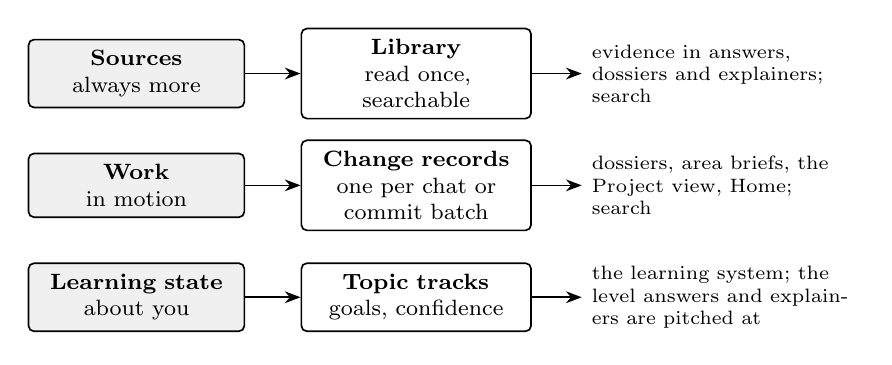
\begin{tikzpicture}[
  kind/.style={draw,rounded corners=2pt,fill=black!6,align=center,inner sep=4pt,text width=7em},
  store/.style={draw,rounded corners=2pt,align=center,inner sep=4pt,text width=7.5em},
  use/.style={align=left,text width=9.5em,font=\scriptsize}]
\node[kind] (src) {\textbf{Sources}\\always more};
\node[kind,below=1.6em of src] (work) {\textbf{Work}\\in motion};
\node[kind,below=1.6em of work] (learn) {\textbf{Learning state}\\about you};
\node[store,right=2em of src] (lib) {\textbf{Library}\\read once, searchable};
\node[store,right=2em of work] (rec) {\textbf{Change records}\\one per chat or commit batch};
\node[store,right=2em of learn] (tracks) {\textbf{Topic tracks}\\goals, confidence};
\draw[->] (src) -- (lib);
\draw[->] (work) -- (rec);
\draw[->] (learn) -- (tracks);
\node[use,right=1.8em of lib] (u1) {evidence in answers, dossiers and explainers; search};
\node[use,right=1.8em of rec] (u2) {dossiers, area briefs, the Project view, Home; search};
\node[use,right=1.8em of tracks] (u3) {the learning system; the level answers and explainers are pitched at};
\draw[->] (lib) -- (u1);
\draw[->] (rec) -- (u2);
\draw[->] (tracks) -- (u3);
\end{tikzpicture}
\par\medskip\begin{minipage}{0.9\linewidth}\small Every item also carries its area label, so it also feeds that area's brief, which is what working chats read through \texttt{context(area)}. The learning system also draws its teaching material from the library.\end{minipage}
\end{figure}

\Sub{Where your notes sit}
Your notes are the one place the kinds meet, which is why the split felt unclear. A note is a \textbf{source} (you wrote it, it is read into the library), and it is also \textbf{evidence about you}: a lecture note shows what you have covered, so it feeds that course's topic tracks, and a project note feeds that project's brief. In your v3 margin: \you{19 Oct}{notes are very important as context/linking etc.}

\begin{itemize}
\item \textbf{You own the notes repository.} Locus writes into it only with your approval: jots it has filed, and ink exported from the tablet.
\item \texttt{careers/general/} is a folder in it, not a repository of its own.
\item \textbf{Jot} opens where the note belongs: \texttt{Alt-j} from a course's Project view writes into that course's notes, not a generic box \youx{19 Oct}.
\end{itemize}

\Sub{The CV, as the worked case}
The CV is all three kinds at once, which makes it a good test. The repository is \textbf{work}: a light project under Careers, with change records and no dossier. Each release is a \textbf{source}, the latest weighted most: \you{19 Oct}{the history is vital but not as much as the most recent release.} And every claim on it becomes \textbf{learning state} through the ``defend every bullet'' track.

\clearpage
\Sec{3. Links, reframed}

The old links joined documents that shared a word: \texttt{regime}, \texttt{Trade}, \texttt{Order}. You named the fix: \you{19 Oct}{links are more than just words - they should be ideas/decisions/concepts.}

\Sub{What a link joins}
A link joins two \textbf{units of meaning}, each of which is something you could point at:
\begin{itemize}
\item an \textbf{idea}: in Explore, a scout find, a paragraph of your notes;
\item a \textbf{decision}: an entry in a repository's decision log;
\item a \textbf{concept}: a defined thing such as ``sequential Monte Carlo'' or ``Kalman filter'', which a course, a paper and a project can all contain.
\end{itemize}
Links cross all three kinds of information, which answers \you{19 Oct}{are we linking between fixed and living and explore material?}: yes, all of them.

\Sub{How a link is made}
\begin{enumerate}
\item \textbf{Candidates} come from anything new: a change record, a new source, an Explore idea. Each is matched against existing units by meaning and by shared concepts. This step is cheap and runs on everything.
\item \textbf{Judgement.} Claude looks at each candidate pair and keeps it only if it can write the one sentence saying why it matters to you. Most candidates die here, as they should.
\item \textbf{Shown in place.} A link appears only inside something you are already reading: the dossier beside the decision, an answer, a scout find. There is still no link view of its own.
\end{enumerate}

\Sub{Three links this would make (illustrative)}
\begin{itemize}
\item Your Control lecture 8 note on regime filtering $\to$ nabla's decision to drop the momentum family: ``the filter you covered on 14 Oct is the tool the D7 re-check asks for.''
\item A scout find on Bayesian optimisation $\to$ QUAST D14 (compass search): ``reports 3$\times$ fewer measurements on a similar device; worth re-checking D14.''
\item The tanker-flow Kalman nowcast idea in Explore $\to$ the Optimisation course: ``the course's week 6 covers the filter this idea needs.''
\end{itemize}
None of these could come from shared words: the first pair shares no word at all.

\Sub{What happens to the old engine}
\you{19 Oct}{is the old engine even worth keeping?} Yes, for one job: reading PDFs with maths and figures into searchable text, which is hard and already works. Its nightly word-matching links are retired; the new linking job replaces them. It is built after the dossier loop, because it feeds on change records \prop. Your decision network, \you{19 Oct}{decision network/graph would be interesting to view}, grows out of it later, in the research track.

\clearpage
\Sec{4. What your v3 markup changed}
Recorded here so the plan is final; these go into the copy of the plan kept in the repository when building starts.
\begin{itemize}
\item \textbf{One system:} \you{19 Oct}{all linked together to form one system that knows about everything.} That is Parts 1 to 3 above.
\item \textbf{The learning system} takes interview prep as a subsection, as you drew. You added: \you{19 Oct}{I love that it can be used generally as my own personal course-generator that knows what I am already good at.}
\item \textbf{Area briefs} stay current, and any chat can also fetch more detailed context on demand \youx{19 Oct}.
\item \textbf{Chores} are short things you put off, offered in the gaps, including while you wait on Claude: \you{19 Oct}{gap could be waiting for claude, just a small amount of time.} The Project view offers one whenever a session is working.
\item \textbf{Search}: Enter jumps to the result where it lives: the chat at that moment, the note in nvim at that line, the PDF at that page, the decision in Decisions \youx{19 Oct}.
\item \textbf{Ink}: curly brackets are read too: \you{19 Oct}{I also draw curly brackets over the part of a passage that my note refers to, with the point of the bracket often pointing to my note.}
\item \textbf{Canvas} pulls deadlines, PDFs, lectures, notes and course information \youx{19 Oct}.
\item \textbf{Symbols} stay within the theme colours \youx{19 Oct}.
\item \textbf{The desktop} leaves the plan: \you{19 Oct}{not relevant to locus}. The laptop side is tested and sorted \youx{19 Oct}.
\item \textbf{Dropped:} the ``later, if wanted'' list \you{19 Oct}{don't worry about}.
\item \textbf{The new linking job} becomes its own step, after the dossier loop and before the scout, since the scout's links depend on it.
\end{itemize}

\medskip
\you{19 Oct}{otherwise everything feels really good.} Next is building, starting with how the build itself is run, which we settle before Slice 0 begins.

\end{document}
